\subsection{Eksperimenta protokols: FAST FPGA resursu patēriņš un veiktspēja}\label{appx:test3}
\setcounter{table}{0} %Reset table counter for (sub)appendix
\setcounter{figure}{0} %Reset figure counter for (sub)appendix
Eksperimenta mērķis ir novērtēt potenciālo izvirzītā FAST algoritma FPGA modeļa
implementācijas ātrdarbību noskaidrojot resursu patēriņu 
konkrētai parauga FPGA mērķa platformai.
Par parauga FPGA tika izvēlēts Xilinx Virtex-6 (\texttt{XC6VLX75T}), % 6vlx75tff484-3
kuram programmējums tika sintezēts ar Xilinx XST rīku.

\begin{table}[hb]\footnotesize
	\centering
	\caption{FPGA modeļa resursu lietojums un ātrdarbība.}
	\label{tbl:test3-data}
	\vspace{4pt}
	\begin{tabular}{*{7}{c}}
		\toprule
		\input{fpga_test-t1.tbl_tex}
		\bottomrule
	\end{tabular}
	\begin{minipage}{0.5\linewidth}
		\noindent Apzīmējumi:\\
		$N_F$ --- \texttt{fast\_n\_unit} entītijas instanču skaits\\
		$f_\text{clk}$ --- takts frekvence\\
		$B_\text{in}$ --- nepieciešamā datu ieejas caurlaidspēja
	\end{minipage}
\end{table}
\footnotetext{Miljoni pikseļu sekundē.}

Eksperimentā tika sintezēti FAST attēla gabala apstrādes vienības
(\texttt{fast\_n\_chunk\_processor} entītijas) varianti ar pieaugošu
apstrādājamā attēla gabala laukumu. Rezultāti apkopoti
\ref{tbl:test3-data}~tabulā un attēloti \ref{fig:test3-data}~attēlā.
Maksimālā frekvence tika koriģēta, pēc
signālceļa garākās aiztures, jo tika konstatēts, ka sintēzes rīks,
visticamāk nekorekti, noteica maksimālo frekvenci $430.793\units{MHz}$
neatkarīgi no \texttt{fast\_n\_unit} instanču skaita.
\ref{fig:test3-data}~attēlā koriģētie rezultāti attēloti ar tumši zilo
grafiku un (salīdzināšanai) nekoriģētie ar gaiši zilu.

Jāņem vērā, ka sintēzes rezultāti par izmantotajiem resursiem un signāla izplatīšanos
(t.sk.,~maksimālo takts frekvenci) ir tikai aptuvens novērtējums, jo iegūti
pirms ,,resursu izvietošanas'' (\termEn{place and route}) soļa.
Autors uzskata, ka iegūtie dati ir pilnībā adekvāti,
ņemot vērā, ka rezultāti ir paredzēti tikai priekšstata radīšanai par
potenciālo ātrdarbību FPGA platformai.

\begin{figure}[tbh]
	\centering
	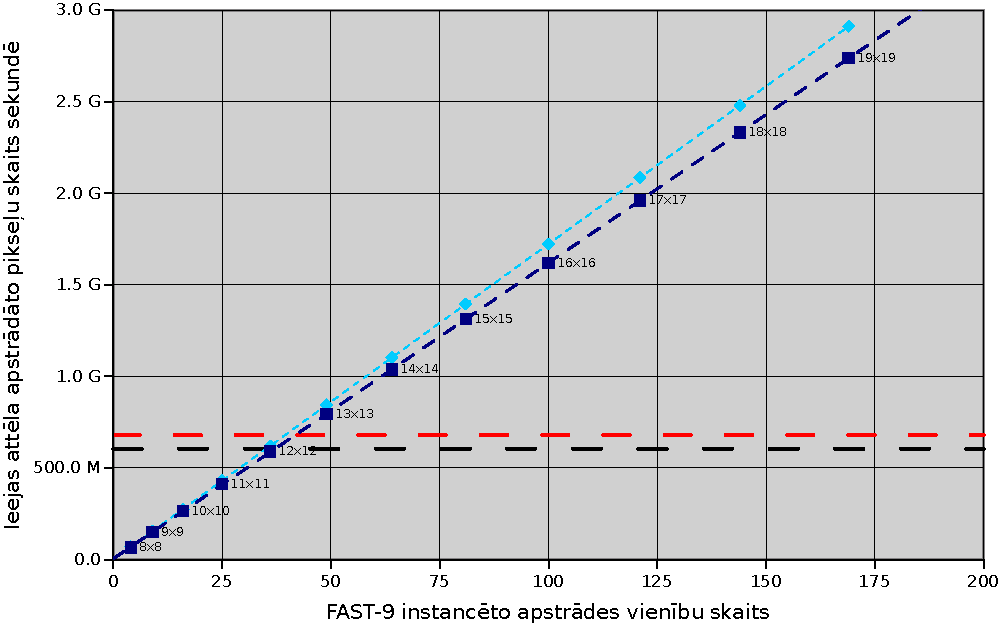
\includegraphics[width=0.9\textwidth]{chart-fpga}
	\caption{Pikseļu apstrādes ātrums pret \texttt{fast\_n\_unit} instanču skaitu.}
	\label{fig:test3-data}
\end{figure}

Pēc rezultātiem var novērot, ka $12 \times 12$ pikseļu gabala apstrāde pie
aptuveni $400\units{MHz}$ takts frekvences sasniedz labākos iegūtos
ātrdarbības rezultātus CPU platformai
(atzīmēts \ref{fig:test3-data}~attēlā ar pārtrauktu, melnu līniju)
izmantojot tikai ceturtdaļu FPGA resursu. Tomēr, lai gan FPGA resursu pietiek
skaitļošanas veiktspējas palielināšanai, šī veiktspēja nav izmantojama, jo
ātrdarbību ierobežo Virtex-6 ātrākās saskarnes (PCI~Express~v2.0~x8)
caurlaidspēja: 20~Gbps (atzīmēts \ref{fig:test3-data}~attēlā ar pārtrauktu,
sarkanu līniju). Var secināt, ka skaitļošanas kompleksitāte salīdzinājumā
ar ieejas datu apjomu nav pietiekami liela, lai panāktu būtisku uzlabojumu
pār CPU. Jānorāda, ka papildus skaitļošana būs nepieciešama raksturpunktu
deskriptoru izveidei un salāgošanai, ko pievienojot ir sagaidāma lielāks
ātrdarbības uzlabojums, jo CPU veiktspēja samazināsies papildus skaitļošanas
dēļ, bet FPGA vēl ir pieejami resursi un papildus skaitļošanu varēs veikt
paralēli FAST algoritmam.
